%----------------------------------------------------------------------------------------
%	PACKAGES AND OTHER DOCUMENT CONFIGURATIONS
%----------------------------------------------------------------------------------------

\documentclass[12pt]{article} % Default font size is 12pt, it can be changed here

\usepackage{geometry} % Required to change the page size to A4
\geometry{a4paper} % Set the page size to be A4 as opposed to the default US Letter

\usepackage{graphicx} % Required for including pictures

\usepackage{float} % Allows putting an [H] in \begin{figure} to specify the exact location of the figure
\usepackage{wrapfig} % Allows in-line images such as the example fish picture
\usepackage{psfrag,amsmath,amsfonts,amsthm,amssymb,cite}
\usepackage{lipsum} % Used for inserting dummy 'Lorem ipsum' text into the template
\usepackage{listings} %for inline code

\linespread{1.2} % Line spacing

\newcommand{\prettycode}[1]
{\lstinline[basicstyle=\ttfamily]{#1}}
\newcommand{\comment}[1]
{\par {\bfseries \color{blue} #1 \par}}



%\setlength\parindent{0pt} % Uncomment to remove all indentation from paragraphs

\graphicspath{{Pictures/}} % Specifies the directory where pictures are stored

\begin{document}

%----------------------------------------------------------------------------------------
%	TITLE PAGE
%----------------------------------------------------------------------------------------

\begin{titlepage}

\newcommand{\HRule}{\rule{\linewidth}{0.5mm}} % Defines a new command for the horizontal lines, change thickness here

\center % Center everything on the page

\textsc{\LARGE CS4516: Final Paper}\\[1.5cm] % Name of your university/college

\HRule \\[0.4cm]
{ \huge \bfseries Tag-Based IP Spoofing Prevention Under Low Deployment Scenarios}\\[0.4cm] % Title of your document
\HRule \\[1.5cm]

\begin{minipage}{0.4\textwidth}
\begin{flushleft} \large
\emph{Author:}\\
Michael Calder\\
Daniel Robertson\\
\end{flushleft}
\end{minipage}
~
\begin{minipage}{0.4\textwidth}
\begin{flushright} \large
\emph{Supervisor:} \\
Dr. Craig Shue % Supervisor's Name
\end{flushright}
\end{minipage}\\[4cm]

{\large \today}\\[3cm] % Date, change the \today to a set date if you want to be precise

%\includegraphics{Logo}\\[1cm] % Include a department/university logo - this will require the graphicx package

\vfill % Fill the rest of the page with whitespace

\end{titlepage}

%----------------------------------------------------------------------------------------
%	TABLE OF CONTENTS
%----------------------------------------------------------------------------------------

%\tableofcontents % Include a table of contents

\newpage % Begins the essay on a new page instead of on the same page as the table of contents 


%----------------------------------------------------------------------------------------
% -- Paper Outline --
% Detail NS-3 implementation of extended protocol, including class and file names. [drob]
% Explain hash-chain and TOTP-based implementation of tag transport [calder]
% Compare and contrast choice of hashing algorithms [calder]
% Talk about hash/security evaluation plan (testing for preimage resistance, ect).[drob]
%----------------------------------------------------------------------------------------

\begin{abstract}
	Shue et. al have developed a robust protocol to prevent IP Spoofing over the Internet. Each implementing router appends a validation tag to packets originating from within their subnet, dropping any packet with a non-conforming IP address\cite{Shue20081567}. However, their underlying mechanism for marking valid packets was shown to be insecure under partial deployment scenarios. As tags are unencrypted, we propose two methods for securing them for transport over insecure channels, so that intercepted packets do not leak any tags. We show that our extension to the original protocol protects the packet tag mechanism, while adding only a negligible computational overhead.

\end{abstract}

\section{Introduction}

A critical vulnerability exists within the very threading of the Internet. Our world's backbone for digital information exchange focuses naively on the receiver of a transmission, without giving proper regards to who the sender is. Malicious attackers exploit this short sight in order to temporarily disable target servers by issuing more requests then the target can handle, a technique known as denial of service (DoS). An attacker who rapidly alters, or spoofs, the source IP address on traffic they generate cannot be tracked. Existing counter measures attempt to mitigate the effect of DoS attacks on the server, but fail to address the underlying issue at hand. 

\subsection{Background and Motivation}
Shue et. al propose an eloquent solution which effectively curbs IP spoofing at the source. In their approach, implementing routers inspect the source address of each packet, and ensure that it is a conforming address with respect to their subnet\cite{Shue20081567}. Explicitly, if this router's subnet was 130.215.0.0/16 (that of the university this research was conducted under), and an encountered outgoing packet had a source IP of 176.230.1.5, the packet would be dropped. Should inspection pass, a unique tag (known by each other implementing router) which identifies the particular router, is added to the packet. Each downstream router en route to the destination checks for the presence of such a tag, and adds its own if one is found. Their analysis proves that their protocol is able to deny spoofed IP packets from entering the larger network at a rate nearing 100\%. The catch, however, is that this effectiveness is contingent on a high deployment status

Shue et. al note that the integrity of a given packet tag is weak under topologies with partial protocol deployment. A compromised tag threatens to undermine the efforts of the IP Spoofing prevention. Their own analysis shows that when only 10\% of the network implements their anti-spoofing protocol, then 66\% of networks can abuse a leaked tag (assuming 100\% collusion)\cite{Shue20081567}. As the cost of changing router functionality to implement the protocol is likely to deter deployment speeds, the problem of tag theft may discourage adoption.

In an effort to smooth out the tag security concerns which emerge under low deployment scenarios, we propose two methods to secure the underlying packet tag implementation. Both combine a fast non-cryptographic hash algorithm (xxHash) with a nonce derived from the current unix time. By mending tag security concerns under low deployment, our modifications add further incentive to early adoption.

\subsection{Related Work}
Many approaches to preventing inter-domain IP spoofing (where attackers attempt to spoof IP addresses outside of their personal domain), already exist. Most prominent are those which attempt to trace the route of the attacking packet back to the (true) source, such as \cite{Taylor}. Shue et. al's approach follows more along the lines of packet filtering, ie. dropping packets near or around the source. Research such as \cite{rfc2827} perform ingress filtering, which drop spoofed packets from within the originating network, but fail to cover packets that escape into the wild.

\section{Methodology}

Our implementation and evaluation was done through the Network Simulator 3 (NS-3) framework. NS-3 is an extensive open source framework for network testing and simulation, written in C++ with Python bindings for higher level scripting. It's seen wide spread use in both commercial and academic pursuits. After learning the NS-3 way of doing things, implementing a novel networking protocol is relatively straight forward. As was the case with this project, simply forking the repository, and extending a few base classes with the desired functionality, allows for rapid development.

\begin{figure}[ht!]
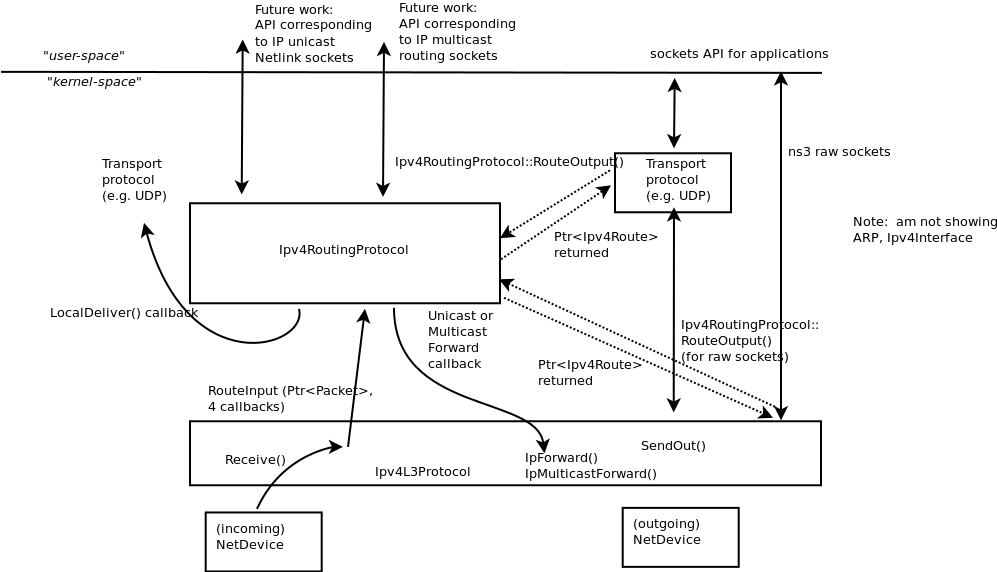
\includegraphics[width=160mm]{routing.png}
\caption{NS-3 \prettycode{Ipv4RoutingProtocol} diagram. Note the interaction between the simulated layer's through RouteInput and RoutOutput\cite{ns-3-routing}}
\end{figure}

Since our extended protocol operates on the network layer, we worked mainly with NS-3's \prettycode{Ipv4RoutingProtocol} interface. We extended the Ipv4GlobalRouting implementation in order to perform the necessary tag protocol logic on a per packet level. The \prettycode{Ipv4RoutingProtocol} expects a RouteInput and RouteOutput function to be specified, which handles the control logic of prefix matching and packet forwarding. Here, we created a tag table as specified in \cite{Shue20081567}. Since our project's focus is more on the exchange of tagged packets over an insecure connection, we assumed that each router's tag table would already be populated. We did this by deterministically calculating a router's tag based off its associated prefix and incoming interface. This allows each router to act as though it's been fully configured, without the added implementation of tag discovery. 

\subsection{Incorporating tags into NS-3}

Tags are stored within each packets header as a a list of tag objects. Necessary interaction functions (add, get, remove) were added to the \prettycode{ipv4-header} class to support the addition of a tag field. The RouteInput and RouteOutput hooks both receive a Packet and Header pointer, allowing for this tag data to be accessed and modified by each router in the stream. 

These modifications are still insufficient to emulate our extended protocol in an actual deployment simulation. At its core, an NS-3 simulation manages a group of configurable objects called \prettycode{Nodes}. A Node can act as an end host, but can also be further extended to include a \prettycode{NetDevice} (analogous to an NIC) in order to function as a router. \prettycode{Nodes} are allocated and managed by \prettycode{NodeContainers}. We used these containers to logically divide multiple \prettycode{Nodes} into Subnets, each with their own tag. Client Nodes within the subnet are connected over \prettycode{CSMA} (forming a bus topology). The edge router in each subnet is attached to the main network over a \prettycode{PointToPoint} link. Each router node is configured before simulation start up by the \prettycode{GlobalRouteManager} class. We hooked into the configuration process in this class to control the deployment status of our extended protocol on each router. Each node manages an instance of the \prettycode{GlobalRouter} class (which uses the \prettycode{Ipv4GlobalRoutingProtocol}), allowing it to function as a router. Since the \prettycode{Ipv4RoutingProtocol} is designed to work independently of per router information (such as the routers IP address), the \prettycode{GlobalRouter} class has to communicate this information to the Node's \prettycode{Ipv4RoutingProtocol} object. This is what allows each router to know and add its subnet's tag to the packet. The extended protocol is disabled by default in our modified \prettycode{Ipv4GlobalRoutingProtocol} class, so it must be manually enabled via the \prettycode{GlobalRouter}. When the simulation begins, all Nodes are iterated over, and those with a \prettycode{GlobalRouter} object aggregated to them are assigned to the protocol depending on the result of a call to \prettycode{rand} compared against a deployment threshold.

Just as in a normal network, information is encapsulated in {\prettycode Packets}, wrapped in a number of {\prettycode Headers}. While in an ideal network, the tags would be implemented in the IP Header, for the sake of convenience, we chose instead to attach the tags to the {\prettycode Packet} class. The class exposes an API for adding attributes to simulated packets that persist throughout their transmission. Interestingly enough, these are simply called {\prettycode Tags}. Our protocol tags are therefore an extension of NS-3's Packet {\prettycode Tag} interface.

With a stable modified implementation of the \prettycode{Ipv4RoutingProtocol} and its constituent classes, we set up a small topology consisting of multiple different subnets. This novel topology consists of two simulated LANs each with an edge router, attached to each other over two different intermediary routers (each with their own subnets). The ensures that each packet passes through at least two tagging routers. A UDP echo client/server application is installed on each client Node, allowing back and forth communication over our protocol. Here, we focused on the generation and verification of secured packet tags, based off of a router's base tag. We devised two core approaches, both of which involve computing the hash of a base tag in order to combine it with the current unix time interval. Both these approaches aim to vary the output tag that is to be transfered over an insecure channel, such that an attacker who obtains it cannot use it to spoof routers inside its originating subnet.

\subsection{Adding security to the tag system}

We tested both the speed and security of two different approaches to preventing tags from being compromised. For each of these approaches, we used and compared both the fastest known non-cryptographic hash function (xxHash\cite{xxhash}) and one of the fastest known cryptographic functions (SHA-1). 

The first approach is hash-chaining, which involves producing a series of hashes of the original tag to be used each day (changing the seed each day so that no two days have the same hash series). Every hash is the previous digest hashed again. If the time interval that these hashes change each day is 30 seconds, then we would need to produce 2,280 hashes to be stored in the router's RAM each day. We tested how long it took to brute-force each hash algorithm, in order to decide the maximum time interval that can be used and still render a compromised hash useless after its time interval has ended. We measured how reasonable the needed memory is for each algorithm and how long it takes for routers to produce each day's chain. We note that for this approach, xxHash is a more attractive option, as it would allow large chains of small 32 bit hashes to be computed relatively quickly.

The second approach is inspired by TOTP (Time-based One-time Password)\cite{rfc6238}. We combine the current time (rounded to some interval like 30 seconds) with the original tag and then hash that result, rendering compromised hashes only useful for a small time interval. Security is a more important factor in this approach because given a time in addition to the hash algorithm, an attacker may be able to obtain the original tag. We analyzed the pre-image resistance of the output using a traditional brute-force approach, in order to determine the resilience of the approach. Clearly, it should be computationally difficult to derive the base tag from a hashed tag, when given the time interval used at the time of hashing, and the hash function its self. This calls for a cryptographic hash function, so we anticipate that SHA-1 and stronger cryptographic functions will be more secure. 

We measured the number of hashes that can be computed over a one second time span for both algorithms. In addition, we examined the space complexity associated with the hash-chaining method, particularly the amount of storage required for one day's worth of generated tags. Finally, we analyzed whether tag creation and authentication incurs latency overhead at each router in the topology (to be measured in milliseconds). As given in the results section, we considered our approach successful, as this difference was under a millisecond, using either hashing method.

\section{Results}

After implementing the hash-chain and TOTP-inspired protocols using NS-3, analysis of the results has shown that both methods offer significant security benefits without causing problems with performance. Each of the two approaches has its own advantages; in this section we will examine these differences and explain how each of the hash functions affect security and performance. The time interval we used for both methods was about half a minute (32 seconds) but could easily be adjusted to add security or space-efficiency. We chose this time interval because we were never able to crack any collisions in less than half a minute when attempting to brute force a hash. 

\subsection{Evaluation of the two methods}

With the hash-chain approach, a compromised hash can only be exploited within the duration of the time interval it was created with. Also, no matter how many hashes we captured, we were not able to determine the original tag (mostly due to collisions) which prevents an attacker from determining future hashes. The only downside of this approach is space complexity. If the interval is roughly half a minute and one day of hashes are generated at a time, 2880 hashes (11KB for xxHash, 46KB for SHA-1) must be stored in RAM. These amounts are not beyond the capabilities of popular routers, but obviously requiring one fourth the space is preferable. Note that as the time interval gets smaller, these numbers grow significantly. Using a 128-bit hash like SHA-1 will also use up four times as much memory as a 32-bit hash like xxHash. With that said, these issues can be negated by increasing how often the hashes are generated (i.e. twice a day).

For the TOTP-inspired approach, each compromised hash also proved useful for a maximum of 32 seconds and then became useless. Because the original tag cannot easily be determined due to collisions (even if the method for combining the timestamp with the tag is known), this method also made stolen hashes unhelpful to attackers in predicting future hashes. Almost no additional memory is needed for this approach and the time interval can be adjusted as desired. The downside to this approach is that, with a lot of work, the original tag can be determined. Using rainbow tables, knowledge of how the timestamp is combined with the tag, and a lot of CPU, having multiple compromised hashes and timestamps can allow an attacker to determine the original tag by comparing the brute-force results until there is only one common tag in the lists of collisions. With that said, breaking this system now becomes time-intensive to acquire only one tag.

\begin{figure}[ht!]
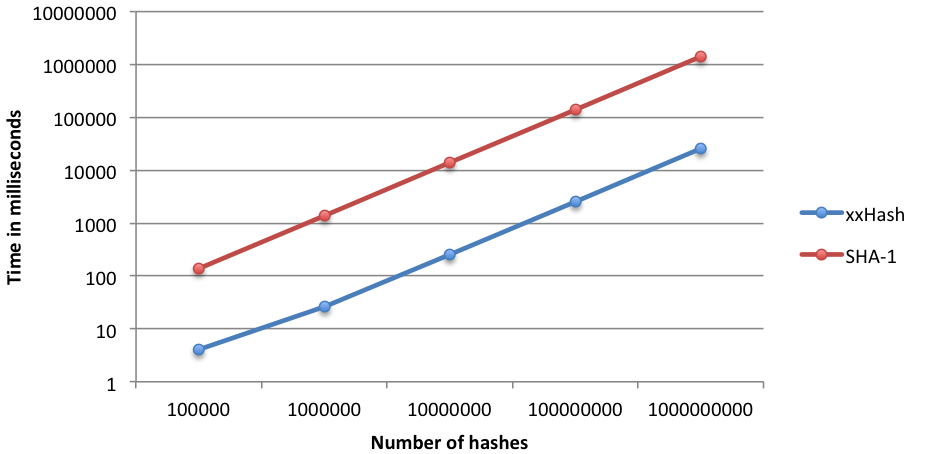
\includegraphics[width=160mm]{hashspeeds.png}
\caption{Hash speeds for xxHash and SHA-1 on a 2.4GHz processor}
\end{figure}

The main differences between cryptographic and non-cryptographic hash functions seemed to be the speed. xxHash, being the fastest non-cryptographic hash algorithm, ran up to 40 million hashes per second. SHA-1, being one of the fastest cryptographic hash algorithms, maxed out around 728 thousand hashes per second. In practice, xxHash caused no measurable latency in the test network (same total time in milliseconds for tag creation/authentication in each router) while SHA-1 failed to meet this requirement. For the once-a-day calculations required for hash chaining, the speeds (on a 2.4GHz processor, which was used to simulate the network) are shown in Figure 1. As far as security is concerned, rainbow tables render both algorithms just as difficult to brute-force. When the original tag is 48 bits, almost 300 trillion possibilities need to be iterated through before a list of all possible original tags that could produce a given hash is known.

So why not use xxHash in any context? xxHash is not a cryptographic hashing algorithm because it is not second preimage resistant, which means that it is possible to determine potential collisions without using brute-force methods. This can be insecure in some contexts, but for what we are trying to accomplish it does not cause an issue because collisions cannot be leveraged. If anything, more collisions only complicate the process of attempting to reverse each hash in a hash chain or trying to determine the original tag from a TOTP-inspired hash. For the purposes of making compromised tag-hashes not a security concern, we have concluded that both of our approaches (using xxHash) are effective and have the potential to provide any reasonable desired space and time efficiency.

\section{Future Work}

We suggest additional security measures, which when combined with our modifications, would further the strength of Shue et. al's protocol. As the protocol is plug and play, the base tags must be distributed over the network before they can be used. This exposes the raw tags during initial deployment, and threaten to undermine our efforts of securing the tags in subsequent exchanges. The initial dispersion of these tags could therefore benefit from encryption. A na\"{i}ve approach would be to use Public key infrastructure, encrypting with the recipient router's public key. However, as noted by Shue et al., the overhead associated with cryptographic operations would severely limit packet throughput. 

\section{Conclusion}

Our research adds a lightweight security layer on top of the packet tagging protocol proposed by Shue et. al. In a realistic scenario where deployment is slow, tag theft presents ample opportunity for circumventing the spoofing measures. We have shown through our analysis that hashing base tags for transportation renders compromised tags unusable. By using hash chains constructed through a very fast non-cryptographic algorithm, we ensure that the tag exchange does not become stale. Our contributed implementation allows tag hashes to be generated and authenticated at a speed of 40 million hashes per second, with no space overhead when using our TOTP-inspired protocol. We have shown that this simple extension of Shue et. al's original protocol will mend initial tag security concerns. We expect that this will further incentivize initial adoption of the original protocol.




%----------------------------------------------------------------------------------------
%	BIBLIOGRAPHY
%----------------------------------------------------------------------------------------

\bibliography{references.bib}
\bibliographystyle{unsrt}

%----------------------------------------------------------------------------------------

\end{document}
